                                                                                                                                                                                                                                                     \documentclass{article}
\usepackage{amsmath}
\usepackage{amsthm}
\usepackage{amssymb}
\usepackage{algorithm}
\usepackage{graphicx}
\usepackage[noend]{algpseudocode}

\newlength\tindent
\setlength{\tindent}{\parindent}
\setlength{\parindent}{0pt}
\renewcommand{\indent}{\hspace*{\tindent}}

\newtheorem{thm}{Theorem}
\newtheorem{cor}{Corollary}[thm]
\newtheorem{lemma}{Lemma}[thm]

\title{Sequence Alignment Problem}
\author{Daniel Braithwaite}

\begin{document}
	\pagenumbering{gobble}
	\maketitle
	\newpage
  	\pagenumbering{arabic}
  	
  	\section{Optimal Substructure}
  		We think of our sequence alignment for strings $x$ of length n and $y$ of length m as a matching between the sets $\{1,....,n\}$ and $\{1,....,m\}$. For any matching $M$ between the two sets to be an alignment it must not contain any crossing pairs\footnote{Algorithm Design Pg 280}
  		
		\begin{align*}
  			if\ (i,j),(i^\prime, j^\prime)\  \in M\\
  			then\ i < i^\prime\ and\ j < j^\prime
  		\end{align*}  		
  		
		We start by making the following observation\footnote{Algorithm Design Pg 281}
		
		\begin{align*}
			ether\ (n, m)\ \in M\\
			or\ (n, m)\ \not\in M
		\end{align*}		 	
		
		Either the last characters of the strings $x$ and $y$ are matched or they are not, this isn't very helpful, but we can say the following
		
		\begin{thm}
				Let M be any alignment of the strings $x$ and $y$.
				If $(n,m) \not\in M$ then ether the $m^{th}$ position of $x$ or the $n^{th}$ position of $y$ is not matched\footnote{Algorithm Design Pg 281}.
		\end{thm}
		
		\begin{proof}
			Suppose for a contradiction that $(n,m) \not\in M$ and there are numbers $i < n$ and $j < m$ such that $(n,i) \in M$ and $(j, m) \in M$. This is a contradiction as we assumed M was an alignment of the strings $x$ and $y$ but we have $(n,i),(j,m) \in M$ where $i < n$ but $j > m$ so the pairs cross and M can not an alignment.
		\end{proof}
		
		We can re write this theorem as the following\footnote{Algorithm Design Pg 281}
		
		\begin{cor}
			In an optimal alignment M, one of the following must be true
			
			\begin{enumerate}
				\item $(n,m) \in M$
				\item The $n^{th}$ position in X is not matched
				\item The $m^{th}$ position in Y is not matched
			\end{enumerate}
		\end{cor}
		
		\begin{lemma}
			The sequence alignment problem has optimal substructure
		\end{lemma}
		
		\begin{proof}
			Let $x$ of length n and $y$ of length m be two strings and let $x^\prime$ and $y^\prime$ be the optimally aligned strings. We know one of the following must be true so we will show optimal substructure holds in all cases.
			
			\begin{enumerate}
				\item $(n,m) \in M$, assume for a contradiction that $x^\prime - \{x_n\}$ and $y^\prime - \{y_m\}$ isn't the optimal solution for the strings $x - \{x_n\}$ and $y - \{y_m\}$. But then we could get a better alignment $a$, $b$ such that $a \cup \{x_n\}, b \cup \{y_m\}$ is an better alignment for $x, y$. This is a contradiction as $x^\prime$ and $y^\prime$ where already optimal
				
				\item The $n^{th}$ position in X is not matched, assume for a contradiction that $x^\prime - \{x_n\}$ and $y^\prime$ isn't the optimal solution for the strings $x - \{x_n\}$ and $y$. But then we could get a better alignment $a$, $b$ such that $a \cup \{x_n\}, b$ is an better alignment for $x, y$. This is a contradiction as $x^\prime$ and $y^\prime$ where already optimal.
				
				\item The $m^{th}$ position in Y is not matched, assume for a contradiction that $x^\prime$ and $y^\prime - \{y_m\}$ isn't the optimal solution for the strings $x$ and $y  - \{y_m\}$. But then we could get a better alignment $a$, $b$ such that $a, b \cup \{y_m\}$ is an better alignment for $x, y$. This is a contradiction as $x^\prime$ and $y^\prime$ where already optimal.
			\end{enumerate}
		\end{proof}
  		
  	\section{Greedy Algorithm}
  		At any point in the string we only need to look at the current 6 characters (the characters $x_i$, $x_{i+1}$, $x_{i+2}$ and $y_j$, $y_{j+1}$, $y_{j+2}$) to make an optimal decision at that point. This is because to balance out a space inserted in one of the strings we need the two after it to match up. We want to be able to look at these characters and decide if we put a space at $i$ in the string $x$ or $j$ in the string $y$. Therefore we layout the characters like below and there are 4 cases that we are interested in\newline\newline
  		
  		\textbf{NOTE:} Here we will refer to the "local score" as the score of the 6 characters by them selves.
  		
  		\begin{center}
  			\begin{tabular}{ c c c }
  				$x_i$ & $x_{i+1}$ & $x_{i+2}$\\
  				$y_j$ & $y_{j+1}$ & $y_{j+2}$\\
  			\end{tabular}
  		\end{center}
		
		\begin{enumerate}
		
			\item \textbf{Last two are equal} $x_{i+2} = y_{j+2}$. Here we don't want to add any spaces as no matter which of the following 3 cases occur if $x_{i+2} = y_{j+2}$ then adding a space will ether make the local score worse or not change it at all. Unless we are in case 2. 
			
			\item \textbf{First four are equal} $x_i = y_j$ and $x_{i+1} = y_{j+1}$	here we have a local score of 1. There is no way that adding a space will improve this, even if we also have a occurrence of case 3 this will just keep the score unchanged at 1. Here if we also have an occurrence of case 1 then it is easy to see that we wouldn't want to add any spaces as the string at this point lines up perfectly
			
			\item \textbf{Double diagonal match} one example of this case $x_i = y_{j+1}$ and $x_{i+1} = y_{j+2}$. Here we want to align the rows, in the example this means that we want to add a space to the string $x$. This will take the local score from -3 to 0. Here if the last two are the same then we would have a local score of -1 at worst and adding a space would still take us to 0.
			
			\item \textbf{Single diagonal match} one example of this case $x_i = y_{j+1}$ and $x_{i+1} != y_{j+2}$. Here we want to align the rows like in case 2. So as before in the example this means adding a space to $x$. This would take the local score from -3 to -2. Here if the last two are equal then the local score would be -2 and adding a space would take us -3 
		\end{enumerate}
	
		Now that we know what to look for we can build an algorithm around these cases. We see that the algorithm follows the optimal substructure as at any point we can think of our current position in the strings as the end of them and we are deciding weather too match them or add a space		
		
		\subsection{Algorithm}
			\begin{algorithm}
				\begin{algorithmic}[1]
					\Procedure{greedyStringAlign}{$x, y$}				
						\State $x^\prime \gets ""\ y^\prime \gets ""$
					
						\State $i \gets 0, j \gets 0$

						\While{$i < x.length\ or\ j < y.length$} \Comment{While we haven't reached the end of one of the strings}
							\If{$i == x.length\ or\ (x[i] = y[j+1]\ and\ x[i+1] = y[j+2])$}
								\State Add space to $x^\prime$
								\State Add $y[j]$ to $y^\prime$
								\State $j \gets j+1$
							
							\ElsIf{$j== y.length\ or\ (x[i+1] = y[i] and x[i+2] = y[i+2])$}
								\State Add $x[i]$ to $x^\prime$
								\State Add space to $y^\prime$
								\State $i \gets i+1$						
						
							\ElsIf{$x[i+2] = y[i+2]$}
								\State Add $x[i]$ to $x^\prime$
								\State Add $y[j]$ to $y^\prime$
								\State $i \gets i+1, j \gets j+1$					
						
							
							\ElsIf{$x[i] != y[i]\ and\ x[i+1] != y[i+1]$}
								\If{$x[i] = y[j+1]$}
									\State Add space to $x^\prime$
									\State Add $y[j]$ to $y^\prime$
									\State $j \gets j+1$
								
								\ElsIf{$x[i+1] = y[i]$}
									\State Add $x[i]$ to $x^\prime$
									\State Add space to $y^\prime$
									\State $i \gets i+1$
								\EndIf
							\EndIf
						
						\EndWhile
						
						\Return $\{x^\prime, y^\prime\}$				
					
					\EndProcedure
					
				\end{algorithmic}
			\end{algorithm}			
			
			\subsection{Analysis}
				In the worst case for this algorithm, only increment one of $i$ or $j$ for each iteration of the loop. Giving a total number of steps as $x.length + y.length$ and thus making the complexity of the algorithm
				
				\begin{align}
					O(x.length + y.length)
				\end{align}
	
			
			\subsection{Example Of Failure}
				The greedy algorithm provides a correct result but the result isn't always optimal. An example of this is if you give it the following two input strings $x = GTAC$ and $y = CAGT$ the greedy algorithm produces the following output
		
				\begin{center}
					\begin{tabular}{ c c c c c }
						G & T & A & C & \\
						C &  & A & G & T
					\end{tabular}
				\end{center}						
  				
  				This alignment has a score of -5 but it is possible to get a better alignment which has a score of -4
  				
  				\begin{center}
					\begin{tabular}{ c c c c }
						G & T & A & C \\
						C & A & G & T
					\end{tabular}
				\end{center}				
			
			\break			
			
			\section{Dynamic Algorithm}
			
				To create a dynamic algorithm we must have a recurrence so we can find a solution in terms of sub problems. For two input strings $x$ and $y$ we let T denote the table of solutions (so $T[a][b]$ is the cost of aligning the strings $x[0:a]$ and $y[0:b]$, and $C_{i,j}$ be the cost of aligning the characters $x_i$ with $y_j$.
				
				\[max
					\begin{cases}
						T_{i-1, j-1} + C_{i,j}\\
						T_{i-1,j} + 2\\
						T_{i, j-1} + 2
					\end{cases}
				\]
				
				This algorithm respects the optimal substructure defined in question 1 as the recurrence the algorithm uses to compute each of the solutions respects the optimal substructure.
					
					We see that for two strings $x$ and $y$ when we are at position $i$ in $x$ and $j$ in $y$ the score optimal solutions for the strings $x[0:i]$ and $y[0:j]$ is defined as the max of the following.
					
					\begin{enumerate}
						\item $T[i-1][j-1] + C_{i, j}$
						\item $T[i-1][j] + C_{space}$
						\item $T[i][j-1] + C_{space}$
					\end{enumerate}
					
					And this is exactly what we showed as the optimal substructure of the sequence alignment problem was.
					
					The part of the table that is filled in before the dynamic algorithm must be correct as we see that the only way to align an empty string with a string of length n is to add n spaces to the empty one, this is what the first one does
			
				\newpage			
			
				\subsection{Algorithm}
					\begin{algorithm}
						\begin{algorithmic}[1]
							\Procedure{dynamicStringAlign}{$x, y$}
								\State $x^\prime \gets ""$
								\State $y^\prime \gets ""$
								
								\State $t \gets [x.length + 1][y.length + 1] of <parent, cost, x, y, type>$
								
								\State Fill out first row of table\Comment{Fill out the parts of the table we already know}
								\State Fill out first column of table
								
								\For{$i \gets 1, i < t.length, i \gets i + 1$}
									\For{$j \gets 1, j < t[i].length, j \gets j + 1$}
										\State $cost \gets $ best cost from recurrence \Comment{Use recurrence to get best next option}
										\State $prevous \gets$ cell based on what the best cost is \Comment{Use recurrence to get the the cell previous cell}
										\State $type \gets$ the type of manipulation we performed
										
										\State $t[i][j] = <previous, cost, i-1, j-1, type>$
									\EndFor
								\EndFor
								
								\State $current \gets t[x.length][y.length]$\newline
								
								\While{$current != null$}
									\If{$current.type\ is\ a\ match$}
										\State $x^\prime \gets x[current.x] + x^\prime$
										\State $y^\prime \gets y[current.y] + y^\prime$
									\ElsIf{$current.type\ is\ a\ space\ in\ x$}
										\State $x^\prime \gets " " + x^\prime$
										\State $y^\prime \gets y[current.y] + y^\prime$
									\ElsIf{$current.type\ is\ a\ space\ in\ y$}
										\State $x^\prime \gets x[current.x] + x^\prime$
										\State $y^\prime \gets " " + y^\prime$
									\EndIf
									
									\State $current \gets current.previous$
								\EndWhile								
								
							\EndProcedure
						\end{algorithmic}
					\end{algorithm}
					
					\break
				
				\subsection{Analysis}
					The algorithm can be split into three sections, the cost of filling out the first row or column, the cost of going through the rest of the table and using the recurrence to fill it out and finally reconstructing the aligned strings.
					
					\subsubsection{Initial Table Setup}
						The cost of filling out one row will be $O(x.length + 1)$ and the cost of filling out one column will be $O(y.length + 1)$ making the total cost $O(x.length + y.length + 2)$
						
					\subsubsection{Calculating Solution}
						Here we are iterating through all of the cells (except the ones in the first row and column). For each of these cells we are doing a constant time operation making the cost $O(x.length * y.length)$
						
					\subsubsection{Finding Aligned Strings}
						In the worst case we would be adding x.length number of spaces to $y\prime$ and y.length spaces to $x^\prime$ so the worst we can do is $O(x.length + y.length)$
						
					\subsubsection{Overall Cost}
						So we have $x.length * y.length + 2*(x.length + y.length + 1)$. This makes the overall cost of the dynamic algorithm
						
						\begin{align*}
  							O(x.length * y.length)
  						\end{align*}
  						
  					\subsubsection{Discussion}
  						For all the cases of some size n (this is when $x.length = y.length = n$) the only part of the algorithm that will effect the running time will be the time to reconstruct the solution. This is because for all the cases it doesn't matter if it is best or worst case the size of the table is the same and we still have to fill it all out. The only difference between the cases is the optimal path through the table. However the cost of reconstructing the solution is $O(x.length + y.length)$ insignificant compared to the cost of building the table $O(x.length * y.length)$.
  						
  			\section{Implementation}
  				In my Java implementation of the dynamic program I am storing the information in a 2D array of tuples. These tuples are of the form $<parent, cost, x, y, type>$. This information will help the aligned sequences be recovered easily.\newline
  				
  				Alternatively I could of made the logic for building the table easier by removing the parent and type but to be able to read the solution from the table it had to be done somewhere and it just seemed nicer to do in the table construction.
  				
  				\subsection{Testing}
  					I ran my algorithm on best, average and worst case input and counted the number of steps it took to fill out the initial bits of the table, fill out the rest of the table and finally reconstruct the solution. I have defined what I mean by best, average and worst case below
  					
  					\begin{enumerate}
  						\item \textbf{Best Case} is when the input strings $x$ and $y$ are identical
  						
  						\item \textbf{Average Case} is just randomly generated problems
  						
  						\item \textbf{Worst Case} not possible to generate as there is no situation where the optimal solution is to add $y.length$ spaces to $x$ and $x.length$ spaces to $y$. As it is cheaper to have two non equal characters that are matched rather than add a space.
  						
  					\end{enumerate}
									
					\begin{figure}[h]
						\vspace{3mm}
						\begin{center}
							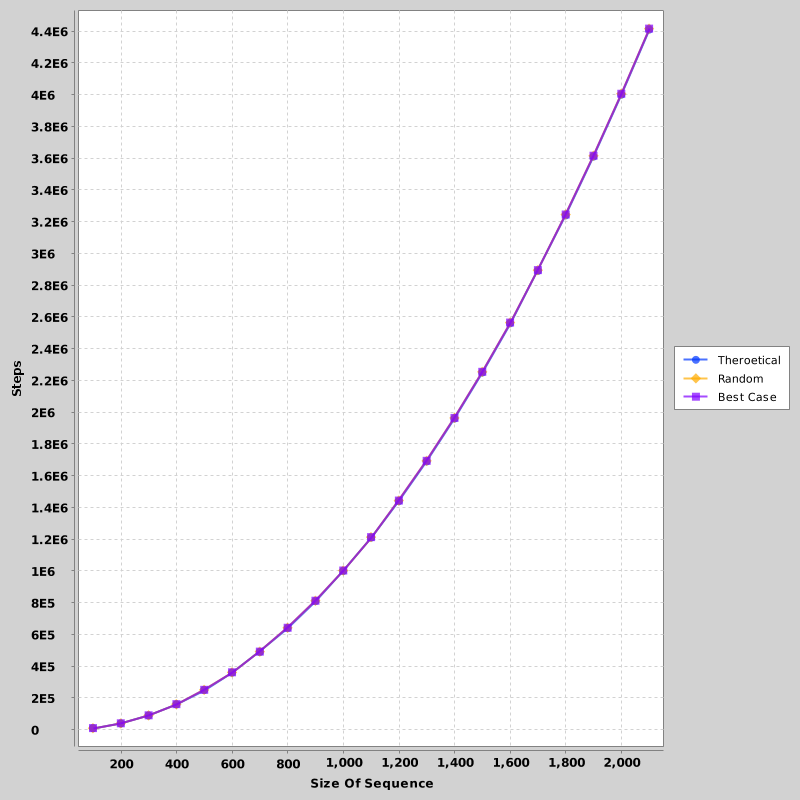
\includegraphics[scale=0.4]{data.png}
						\end{center}
					\end{figure}
					
					
					You can only see one one line in the graph above. This is because as discussed before the only difference between the best and worst case situation is the cost of reconstructing the solution and that is $O(x.length + y.length)$. This is tiny compared to the cost of filing out the table.\newline
					
			\section{Edit Distance}		
				\subsection{Optimal Substructure}
					For the edit distance problem we can think of a solution for input $x$ and $y$ (where we are trying to transform $x$ into $y$) as an alignment of the two strings. Let these be $x^\prime$ and $y^\prime$. A gap in $x^\prime$ we can think of as meaning we are inserting a letter from $y$ into $x$ at that position. A gap in $y^\prime$ we think of as meaning deleting a letter from $x$\footnote{http://mathcs.slu.edu/~chambers/spring09/cs314/schedule/04-dynprog.pdf Pg 4}.\newline
					
					So then we can calculate the cost easily. The number of spaces in $x$ ($S_x$) is the number of insertions. The number of spaces in $y$ ($S_y$) represents the number of deletes performed. The number of matches in the alignment is the number of copy's ($c$) we need to do. Then we will need to count up the mismatches ($m$) in the alignment to find the number of replacements we need to do. Lastly we will need to keep track of the twiddles performed ($t$). Giving us the following formula
					
					\begin{align}
						S_x*C_{insert} + S_y*C_{delete} + c*C_{copy} + m*C_{replacement} + t*C_{twiddle} + C_{kill}
					\end{align}
				
					Just like for the sequence alignment problem we can represent this solution as a matching between the sets $\{1,....,n\}$ and $\{1,....,m\}$. For any matching $M$ between the two sets to be an alignment it must not contain any crossing pairs
  		
		\begin{align*}
  			if\ (i,j),(i^\prime, j^\prime)\  \in M\\
  			then\ i < i^\prime\ and\ j < j^\prime
  		\end{align*} 
					
					Then by the same steps as in section 1 we can see the following
					
					\begin{lemma}
						In an optimal alignment M, one of the following must be true
			
						\begin{enumerate}
							\item $(n,m) \in M$
							\item The $n^{th}$ position in X is not matched
							\item The $m^{th}$ position in Y is not matched
						\end{enumerate}
					\end{lemma}
					
					\begin{proof}
						First lets say that $x_n\ =\ y_m$. Then we don't need to do anything we just leave it. So therefore $(n,m) \in M$.\newline
						
						Now lets say that $x_n \ne y_m$ so then we would perform one of the available actions.
						
						\begin{enumerate}
							\item \textbf{Delete} would remove an element of $x$ meaning that $x_i$ would be unmatched we can think of this as adding a space to $y$ in the $i^{th}$ position
							\item \textbf{Insert} means adding a character to $x$ at some position i. Meaning some position in $y$ wouldn't be matched to a position in $x$. We think of this as adding a space to $x$ in the $i^{th}$ position. 
							\item \textbf{Replace}ing at the $n^{th}$ position in $x$ and the $m^{th}$ position in $y$ inserting a space into the strings so $(n,m) \in M$
							\item \textbf{Copy} Same as replace, means that $(n,m) \in M$
							\item \textbf{Twiddle} This just swaps $x_i$ with $x_{i+1}$ not adding a space so $(n,m) \in M$
							\item \textbf{Kill} at i just removes all the letters after and including i in the string. So for all $k >= i$ $x_k$ is not matched
						\end{enumerate} 					
					
					\end{proof}
					
					\begin{lemma}
						The edit distance problem has optimal substructure
					\end{lemma}
					
					See section 1, lemma 1.1 for the proof as they are identical						
					
				\subsection{Greedy Algorithm}
					Converting our sequence alignment algorithm into something that can solve the edit distance problem is trivial as what we essentially showed in the optimal substructure section was that the edit distance problem is almost like finding the optimal alignment.\newline
					
					What our current algorithm doesn't do is the Twiddle operation. To implement this we just need to check if swapping the current and next character in $x$ around is worth it. This would depend on the cost. For example we might arrive at a position where we can either twiddle or replace, what we do would depend on what costs less. And thus we can calculate the score of the edit distance using (2) in section 5.1
					
					\subsubsection{Complexity}
						The only thing we have added in is checking if the twiddle operation is worth it. This is constant time as we are only comparing the costs of the operations and the elements $x_{i+1}$ with $y_j$. Therefor the complexity of the algorithm will remain $O(x.length + y.length)$
				
				\subsection{Dynamic Algorithm}							
					The dynamic algorithm for this problem would be very similar to the one for sequence alignment. The only difference being the recurrence used. Here we would use
					
					\[cost =	\begin{cases}
						
						T_{i-1,j-1} & a_i = b_i\\
						
						min\begin{cases}
							T_{i-1, j} + C_{delete}\\
							T_{i, j-1} + C_{insert}\\
							T_{i-1, j-1} + C_{replace}\\
							T_{i-1, j-1} + C_{copy}\\
							T_{i-2, j-2} + C_{twiddle}\\
							T_{i-1, j-1} + C_{kill}\\
						\end{cases} & otherwise
						
						\end{cases}
					\]
					
					If we replaced the recurrence in algorithm 3.1 with the one defined above then we would have a dynamic programming algorithm for solving the edit distance problem. The efficiency for two input strings $x$ and $y$ would still be $O(x.length*y.length)$. If we examine the following three sections we will see this.
					
					\subsubsection{Initial Table Setup}
						We haven't changed the size of the table so the cost of filling out one row and one column remains $O(x.length + y.length + 2)$
						
					\subsubsection{Calculating Solution}
						Here we can use the same logic. We haven't changed the size of the table so there are no extra squares to fill out. And changing the recurrence doesn't effect the complexity as these as finding the min of 6 things is a constant time operation. Therefor the complexity for this remains $O(x.length * y.length)$
						
					\subsubsection{Finding Edit String}
						Again we haven't changed the size of the table but the worst case here is a bit different, it occurs if you use delete on all the letters of the string $x$ and then a insert all the letters of $y$. This however still gives the same complexity of $O(x.length + y.length)$
						
					\subsubsection{Overall Cost}
						So we have $x.length * y.length + 2*(x.length + y.length + 1)$. This makes the overall cost of the dynamic algorithm
						
						\begin{align*}
  							O(x.length * y.length)
  						\end{align*}
\end{document}